\documentclass[12pt]{article}
\usepackage{amsmath, amssymb}
\usepackage{graphicx}
\usepackage{float}
\usepackage[letterpaper, margin=1in]{geometry}
\usepackage[colorlinks=true, linkcolor=blue, urlcolor=blue]{hyperref}
\usepackage{listings}
\usepackage{booktabs}
\usepackage{siunitx}
\usepackage{booktabs, xcolor, colortbl, array, caption}
\usepackage{lettrine}
\usepackage{tcolorbox}
\usepackage{bm}

\setlength{\fboxrule}{1.2pt}

\begin{document}
\pagestyle{empty}
\begin{center}
    \Huge \textbf{Analysis}
\end{center}

Now, we'll perform the two-sample t-test for \(\mu_{p} - \mu_{np}\).
\begin{align*}
    t & = \frac{\bar{x}_p - \bar{x}_{np}}{\sqrt{\frac{s^2_p}{n_p} + \frac{{s^2_{np}}}{n_{np}}}}                                       \\
      & = \frac{0.381 - 0.398}{\sqrt{\frac{{(0.335)}^2}{68} + \frac{{(0.290)}^2}{361}}}                                               \\
      & = \frac{-0.017}{0.043397}                                                                                                     \\
      & = -0.3917                                                                                                                     \\[0.5em]
    p & = 2 \cdot \text{tcdf}\Big(\overset{\text{lower}}{-1\text{E}99}, \overset{\text{upper}}{-0.3917}, \overset{\text{df}}{67}\Big) \\
      & = 2 \cdot 0.3483                                                                                                              \\
      & = \boxed{0.6966}
\end{align*}
\begin{figure}[H]
    \centering
    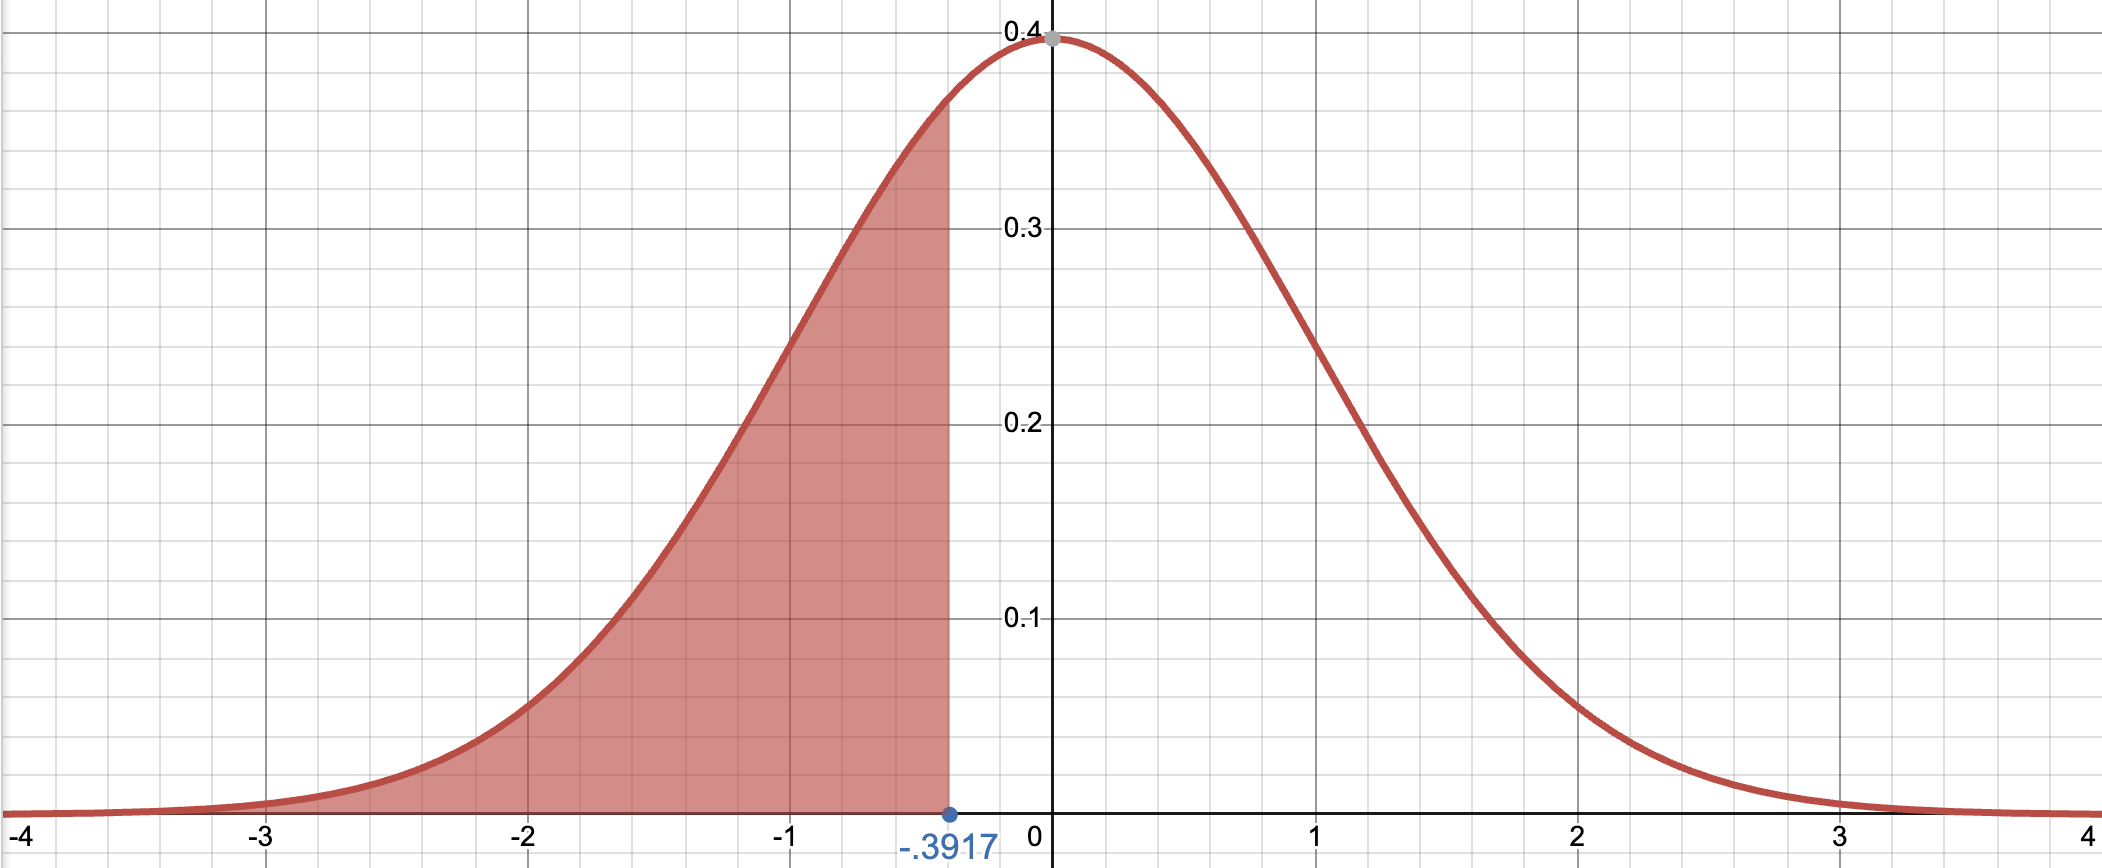
\includegraphics[width=1\textwidth]{tcdf.png}
\end{figure}
Assuming \(H_0\) is true (Shohei's true mean wOBA is the same when pitching vs not pitching), there is a 0.6966 probability of getting a sample with a mean difference as large or larger than the one in this sample (.017).

\textbf{Since \(\bm{p = 0.6966 > \alpha = 0.05}\), we fail to reject \(\bm{H_0}\)}. There is not convincing evidence that Shohei Ohtani's true mean wOBA is different when pitching vs not pitching. This conclusion would hold for any common value of \(\alpha\) (0.01, 0.05, 0.10). This supports my prediction that Shohei would bat similarly regardless of position.

There is a possible type II error, because we failed to reject \(H_0\). This would mean that Shohei actually does bat differently when pitching compared to not pitching. Although a type I error is not possible, as we did not reject \(H_0\), it would mean that Shohei does not bat differently, but we said that he did.

Next, we'll perform a two-sample t-interval for \(\mu_{p} - \mu_{np}\), at confidence level 95\%.
\begin{align*}
    \text{CI} & = (\bar{x}_p - \bar{x}_{np}) \, \pm \, t^* {\sqrt{\frac{s^2_p}{n_p} + \frac{{s^2_{np}}}{n_{np}}}}                                                              \\
              & = (\bar{x}_p - \bar{x}_{np}) \, \pm \, \text{invT}\Big(\overset{\text{area}}{1 - \alpha/2}, \overset{\text{df}}{\text{df}
    }\Big) {\sqrt{\frac{s^2_p}{n_p} + \frac{{s^2_{np}}}{n_{np}}}}                                                                                                              \\
              & = (0.381 - 0.398) \, \pm \, \text{invT}\Big(\overset{\text{area}}{0.975}, \overset{\text{df}}{67}\Big) \sqrt{\frac{{(0.335)}^2}{68} + \frac{{(0.290)}^2}{361}} \\
              & = -0.017 \, \pm \, 1.996 \cdot 0.043397                                                                                                                        \\
              & = -0.017 \, \pm \, 0.08662                                                                                                                                     \\
              & = \boxed{(-0.1036, 0.0696)}
\end{align*}
We are 95\% confident that \((-0.1036, 0.0696)\) contains the true mean difference in wOBA when Shohei is pitching vs not pitching.

Since 0 is on the interval, \(H_0: \mu_p = \mu_{np}\) is plausible. This supports the t-test, in which we failed to reject \(H_0\). The interval gives us a range of plausible values for \(\mu_{p} - \mu_{np}\), showing there is likely a small to zero difference when pitching vs not pitching.
\end{document}
